\documentclass[runningheads]{llncs}

\usepackage[T1]{fontenc}
\usepackage[utf8]{inputenc}
\usepackage{amsmath,amssymb}
\usepackage{booktabs}
\usepackage{listings}
\usepackage{tikz}
\usetikzlibrary{arrows.meta,positioning,shapes.geometric}
\usepackage{url}
\usepackage{hyperref}

\lstset{
  basicstyle=\ttfamily\scriptsize,
  breaklines=true,
  frame=single,
  numbers=left,
  numberstyle=\tiny\color{gray}
}

\begin{document}

\title{From FRET to Range-Checked Zero-Knowledge Proofs: Verifiable Safety Envelopes for Autonomous Deep-Space Habitats}
\titlerunning{From FRET to Range-Checked Zero-Knowledge Proofs}

\author{Sai Sravan Cherukuri\inst{1} \and Sai Saketh Cherukuri\inst{2}}
\authorrunning{S.\ S.\ Cherukuri and S.\ S.\ Cherukuri}
\institute{Independent Researcher / Enterprise \& DevSecOps Architect\\
\email{saisravan@gmail.com}\\
\url{https://github.com/saisravan909/zk-habitat-compliance} \and
AI Performance Engineer, Red Hat\\
\email{ssaketh.2002@gmail.com}}

\maketitle

\begin{abstract}
Autonomous systems in uncrewed or bandwidth-constrained deep-space habitats require verifiable safety assurance without streaming full raw telemetry over constrained links. We present \texttt{zk-habitat-compliance}, an open-source formal-methods tool pipeline linking NASA's Formal Requirements Elicitation Tool (FRET) to a deterministic Python-to-Circom constraint synthesizer (\texttt{fret\_to\_circuit.py}), runtime policy checks, and continuous integration (CI) verification. Across single- and multi-requirement Environmental Control and Life-Support System (ECLSS) specifications (\texttt{HAB-O2-001}, \texttt{HAB-CO2-002}, and \texttt{HAB-VALVE-003}), the translator encodes conditional operational modes via \texttt{IsEqual} comparator guards, prevents finite-field modular wraparound via \texttt{Num2Bits} slack decomposition, and aggregates per-requirement validity flags into a single compliance output. We document the formal R1CS translation semantics, static constraint metrics, synthetic telemetry evaluation, and explicit data provenance separating synthetic validation traces from deferred hardware proving benchmarks.
\end{abstract}

\keywords{Formal Methods \and Tool Paper \and NASA FRET \and Zero-Knowledge Circuits \and Range Checks \and Autonomous Deep-Space Habitats}

\section{Introduction}
Autonomous habitats and deep-space life-support controllers must enforce strict safety envelopes during uncrewed operations and high-latency communication blackouts. Downlinking raw high-frequency sensor logs consumes scarce deep-space bandwidth, whereas unauthenticated status flags lack mathematical assurance that safety invariants actually held over private sensor readings.

To bridge structured requirements engineering with verifiable execution, we introduce \texttt{zk-habitat-compliance}, an open-source prototype that translates structured NASA FRET requirements (\texttt{NASA-SW-VnV/fret}) \cite{fret_repo,fret_ntrs} into range-checked Circom zero-knowledge circuits and executable policy evaluators. Specifically, the tool makes three contributions:
\begin{enumerate}
    \item \textbf{Deterministic FRET-to-Circom Compilation:} Translates single- and multi-requirement JSON exports into sanitized, reproducible Circom 2.1.6 templates with exact \texttt{diff -u} verification in CI.
    \item \textbf{Wraparound-Safe Arithmetic Encoding:} Binds discrete operating modes with \texttt{IsEqual()} comparators and enforces inequality bounds via non-negative slack witnesses constrained by \texttt{Num2Bits(b)} over prime field $\mathbb{F}_p$.
    \item \textbf{Transparent Reproducibility \& Provenance:} Pairs circuit synthesis with a deterministic synthetic telemetry runner (\texttt{scripts/run\_prototype\_check.py}) while explicitly distinguishing synthetic validation inputs from live \texttt{circom}/\texttt{snarkjs} prover benchmarks.
\end{enumerate}

\section{Tool Architecture and Pipeline Workflow}
Figure~\ref{fig:arch} illustrates the end-to-end architecture implemented in \texttt{saisravan909/zk-habitat-compliance}.

\begin{figure}[t]
\centering
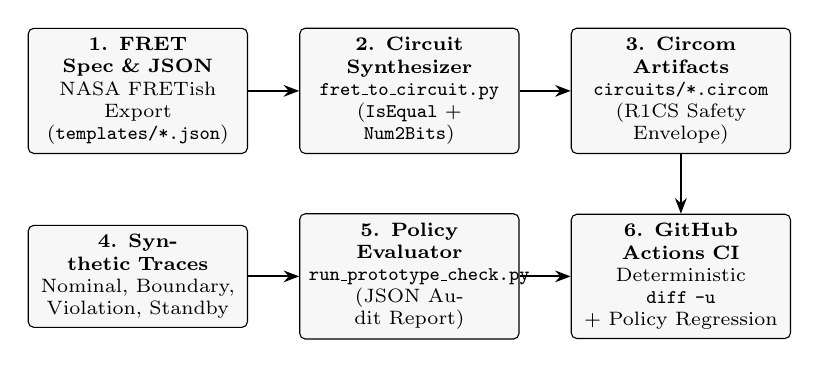
\begin{tikzpicture}[
    node distance=0.85cm and 0.65cm,
    box/.style={rectangle, draw, rounded corners=2pt, align=center, font=\scriptsize, minimum height=0.85cm, text width=2.55cm, fill=gray!6},
    arrow/.style={-{Stealth[scale=0.85]}, thick}
]
\node[box] (fret) {\textbf{1. FRET Spec \& JSON}\\NASA FRETish Export\\(\texttt{templates/*.json})};
\node[box, right=of fret] (trans) {\textbf{2. Circuit Synthesizer}\\\texttt{fret\_to\_circuit.py}\\(\texttt{IsEqual} + \texttt{Num2Bits})};
\node[box, right=of trans] (circom) {\textbf{3. Circom Artifacts}\\\texttt{circuits/*.circom}\\(R1CS Safety Envelope)};

\node[box, below=0.9cm of fret] (sim) {\textbf{4. Synthetic Traces}\\Nominal, Boundary,\\Violation, Standby};
\node[box, right=of sim] (pol) {\textbf{5. Policy Evaluator}\\\texttt{run\_prototype\_check.py}\\(JSON Audit Report)};
\node[box, right=of pol] (ci) {\textbf{6. GitHub Actions CI}\\Deterministic \texttt{diff -u}\\+ Policy Regression};

\draw[arrow] (fret) -- (trans);
\draw[arrow] (trans) -- (circom);
\draw[arrow] (sim) -- (pol);
\draw[arrow] (pol) -- (ci);
\draw[arrow] (circom) -- (ci);
\end{tikzpicture}
\caption{End-to-end workflow of \texttt{zk-habitat-compliance}, linking FRET requirement templates to range-checked Circom circuits, runtime policy checks, and automated CI validation.}
\label{fig:arch}
\end{figure}

The repository organizes artifacts into four modular layers:
\begin{itemize}
    \item \textbf{Requirement Templates (\texttt{fret-extension/templates/}):} Stores structured ECLSS requirements (\texttt{habitat\_o2\_requirement.json} and \texttt{habitat\_multi\_requirements.json}) with integer scaling factors (e.g., $19.5\text{ kPa} \rightarrow 195$) and bit-width bounds (\texttt{bit\_width = 16}).
    \item \textbf{Constraint Generator (\texttt{fret-extension/fretish-to-zksnark/fret\_to\_circuit.py}):} Sanitizes requirement identifiers into valid Circom signals, validates bit widths ($1 \le b \le 252$ for BN254 scalar field safety), emits \texttt{IsEqual()} condition guards, and chains per-requirement validity outputs into \texttt{all\_constraints\_satisfied}.
    \item \textbf{Reference Circuits (\texttt{circuits/}):} Houses committed golden circuits (\texttt{habitat\_o2\_compliance\_ranged.circom} and \texttt{habitat\_multi\_compliance.circom}) verified against fresh generator output on every push.
    \item \textbf{Policy Runner \& CI (\texttt{scripts/} \& \texttt{.github/workflows/}):} Executes deterministic policy evaluation over synthetic telemetry cases and enforces zero-drift circuit generation via \texttt{diff -u}.
\end{itemize}

\section{Formal Encoding and Range Soundness}
Zero-knowledge proof systems such as Groth16 over BN254 operate in a prime finite field $\mathbb{F}_p$ ($p \approx 2^{254}$), where standard integer ordering does not exist: if $v < \tau$, then $(v - \tau) \bmod p = p + (v - \tau)$ wraps around to a large positive field element.

To prevent modular wraparound attacks, \texttt{fret\_to\_circuit.py} compiles each requirement $r_i$ with mode signal $m_i$, target mode constant $\mu_i$, sensor signal $v_i$, threshold $\tau_i$, and bit width $b_i \in [1, 252]$ into Rank-1 Constraint System (R1CS) equations:
\begin{align}
    c_i &= \text{IsEqual}(m_i, \mu_i), \quad c_i \cdot (1 - c_i) = 0, \label{eq:guard}\\
    c_i \cdot ((v_i - \tau_i) - s_i) &= 0 \quad (\text{for } v_i \ge \tau_i), \label{eq:ge}\\
    c_i \cdot ((\tau_i - v_i) - s_i) &= 0 \quad (\text{for } v_i \le \tau_i), \label{eq:le}\\
    c_i \cdot (v_i - \tau_i) &= 0 \quad (\text{for } v_i == \tau_i), \label{eq:eq}\\
    s_i &= \sum_{k=0}^{b_i - 1} 2^k \cdot \beta_{i,k}, \quad \beta_{i,k} \cdot (1 - \beta_{i,k}) = 0. \label{eq:bits}
\end{align}
When mode $m_i = \mu_i$, \texttt{IsEqual} enforces $c_i = 1$, requiring slack witness $s_i = |v_i - \tau_i|$ to decompose into $b_i$ Boolean bits via \texttt{Num2Bits($b_i$)} (Equation~\ref{eq:bits}). Because $2^{b_i} \ll p$, any violating sensor reading ($v_i < \tau_i$ for $\ge$, or $v_i > \tau_i$ for $\le$) yields a field element $p - \Delta \ge 2^{b_i}$ with no valid $b_i$-bit decomposition, rendering the circuit unsatisfiable. When $m_i \ne \mu_i$, $c_i = 0$ vacates Equations~\ref{eq:ge}--\ref{eq:eq}, allowing $s_i = 0$ cleanly. Finally, per-requirement validity flags $w_i$ are combined quadratically:
\begin{equation}
    a_0 = w_1 \cdot w_2, \quad a_{k} = a_{k-1} \cdot w_{k+2}, \quad \texttt{all\_constraints\_satisfied} = a_{n-2}.
\end{equation}

\section{ECLSS Case Study and Static Circuit Metrics}
We evaluate the translator on three autonomous habitat ECLSS requirements specified in FRETish and exported to JSON (Table~\ref{tab:reqs}).

\begin{table}[t]
\centering
\caption{ECLSS Safety Requirements Encoded in \texttt{zk-habitat-compliance}}
\label{tab:reqs}
\scriptsize
\begin{tabular}{l p{5.3cm} c c c}
\toprule
\textbf{Req. ID} & \textbf{FRETish Specification} & \textbf{Op.} & \textbf{Scaled $\tau$} & \textbf{Bits ($b$)} \\
\midrule
\texttt{HAB-O2-001} & In \texttt{habitat\_mode life\_support} shall always satisfy \texttt{o2\_pressure >= 195} & $\ge$ & $195$ & $16$ \\
\texttt{HAB-CO2-002} & In \texttt{habitat\_mode life\_support} shall always satisfy \texttt{co2\_ppm <= 4000} & $\le$ & $4000$ & $16$ \\
\texttt{HAB-VALVE-003} & In \texttt{habitat\_mode life\_support} shall always satisfy \texttt{relief\_valve\_locked == 1} & $==$ & $1$ & --- \\
\bottomrule
\end{tabular}
\end{table}

Table~\ref{tab:circuit_metrics} summarizes the static structural properties of the two deterministic circuits generated by \texttt{fret\_to\_circuit.py} and committed under \texttt{circuits/}.

\begin{table}[t]
\centering
\caption{Static Structural Breakdown of Generated Circom 2.1.6 Circuits}
\label{tab:circuit_metrics}
\scriptsize
\begin{tabular}{l c c c c}
\toprule
\textbf{Generated Circuit Artifact} & \textbf{Reqs.} & \textbf{Private Inputs} & \textbf{\texttt{IsEqual} Guards} & \textbf{\texttt{Num2Bits(16)}} \\
\midrule
\texttt{habitat\_o2\_compliance\_ranged.circom} & $1$ & $3$ & $1$ & $1$ \\
\texttt{habitat\_multi\_compliance.circom} & $3$ & $6$ & $3$ & $2$ \\
\bottomrule
\end{tabular}
\end{table}

\section{Synthetic Telemetry Evaluation and Data Provenance}
To validate requirement semantics and boundary behavior prior to proof generation, \texttt{scripts/run\_prototype\_check.py} evaluates four deterministic synthetic telemetry scenarios against \texttt{HAB-O2-001} ($\tau = 195$). Table~\ref{tab:synth_cases} reports the exact JSON outputs verified in GitHub Actions Run \#18.

\begin{table}[t]
\centering
\caption{Synthetic Telemetry Scenarios Evaluated by \texttt{scripts/run\_prototype\_check.py}}
\label{tab:synth_cases}
\scriptsize
\begin{tabular}{l c c c c l}
\toprule
\textbf{Test Case ID} & \textbf{Mode} & \textbf{O2} & \textbf{Slack} & \textbf{Allow} & \textbf{Evaluator Diagnostic Reason} \\
\midrule
\texttt{nominal\_life\_support} & $1$ & $208$ & $13$ & \texttt{true} & O2 pressure satisfies threshold \\
\texttt{boundary\_life\_support} & $1$ & $195$ & $0$ & \texttt{true} & O2 pressure satisfies threshold \\
\texttt{hypoxia\_violation} & $1$ & $172$ & $0$ & \texttt{false} & VIOLATION: O2 pressure below threshold \\
\texttt{standby\_mode} & $0$ & $150$ & $0$ & \texttt{true} & \texttt{habitat\_mode} inactive; bound not triggered \\
\bottomrule
\end{tabular}
\end{table}

\paragraph{Data Provenance and Benchmarking Scope.}
In accordance with empirical artifact review standards, we explicitly distinguish artifact provenance:
\begin{enumerate}
    \item \textbf{Synthetic Telemetry Inputs:} All sensor values in Table~\ref{tab:synth_cases} are deterministic synthetic test vectors constructed to exercise nominal, boundary, violation, and inactive-mode branches without physical flight hardware.
    \item \textbf{Deferred Prover Timings:} While \texttt{fret\_to\_circuit.py} emits valid Circom 2.1.6 R1CS templates, live \texttt{circom} witness generation and \texttt{snarkjs} Groth16 proving latency/memory measurements are deferred to dedicated hardware runs and are not reported as simulated estimates here.
\end{enumerate}

\section{Artifact Availability and Reproduction}
The complete source code, templates, golden circuits, and CI workflow are publicly available at \url{https://github.com/saisravan909/zk-habitat-compliance}. Reviewers can reproduce circuit synthesis and policy checks directly:
\begin{lstlisting}[language=bash]
python fret-extension/fretish-to-zksnark/fret_to_circuit.py \
  --input fret-extension/templates/habitat_multi_requirements.json \
  --output /tmp/habitat_multi_compliance.circom
diff -u circuits/habitat_multi_compliance.circom /tmp/habitat_multi_compliance.circom
python scripts/run_prototype_check.py
\end{lstlisting}

\section{Conclusion}
\texttt{zk-habitat-compliance} demonstrates an automated, deterministic path from NASA FRET safety specifications to wraparound-safe Circom compliance circuits and runtime policy checks. Future work will integrate temporal sliding-window unrolling across multi-step traces and publish measured \texttt{circom}/\texttt{snarkjs} proving benchmarks on embedded flight-equivalent processors.

\begin{thebibliography}{4}
\bibitem{fret_repo}
NASA Software V\&V: \texttt{fret}: Formal Requirements Elicitation Tool. GitHub, \url{https://github.com/NASA-SW-VnV/fret}.

\bibitem{fret_ntrs}
NASA NTRS: Let's speak FRETish. \url{https://ntrs.nasa.gov/citations/20240004425}.
\end{thebibliography}

\end{document}
